\documentclass[border=10pt]{standalone}

\usepackage{tikz}
\usepackage{tikzsymbols}
\usetikzlibrary{calc,patterns,shapes.geometric}

\def\centerarc[#1](#2)(#3:#4:#5){\draw[#1] ($(#2)+({#5*cos(#3)},{#5*sin(#3)})$) arc (#3:#4:#5);}

\begin{document}
	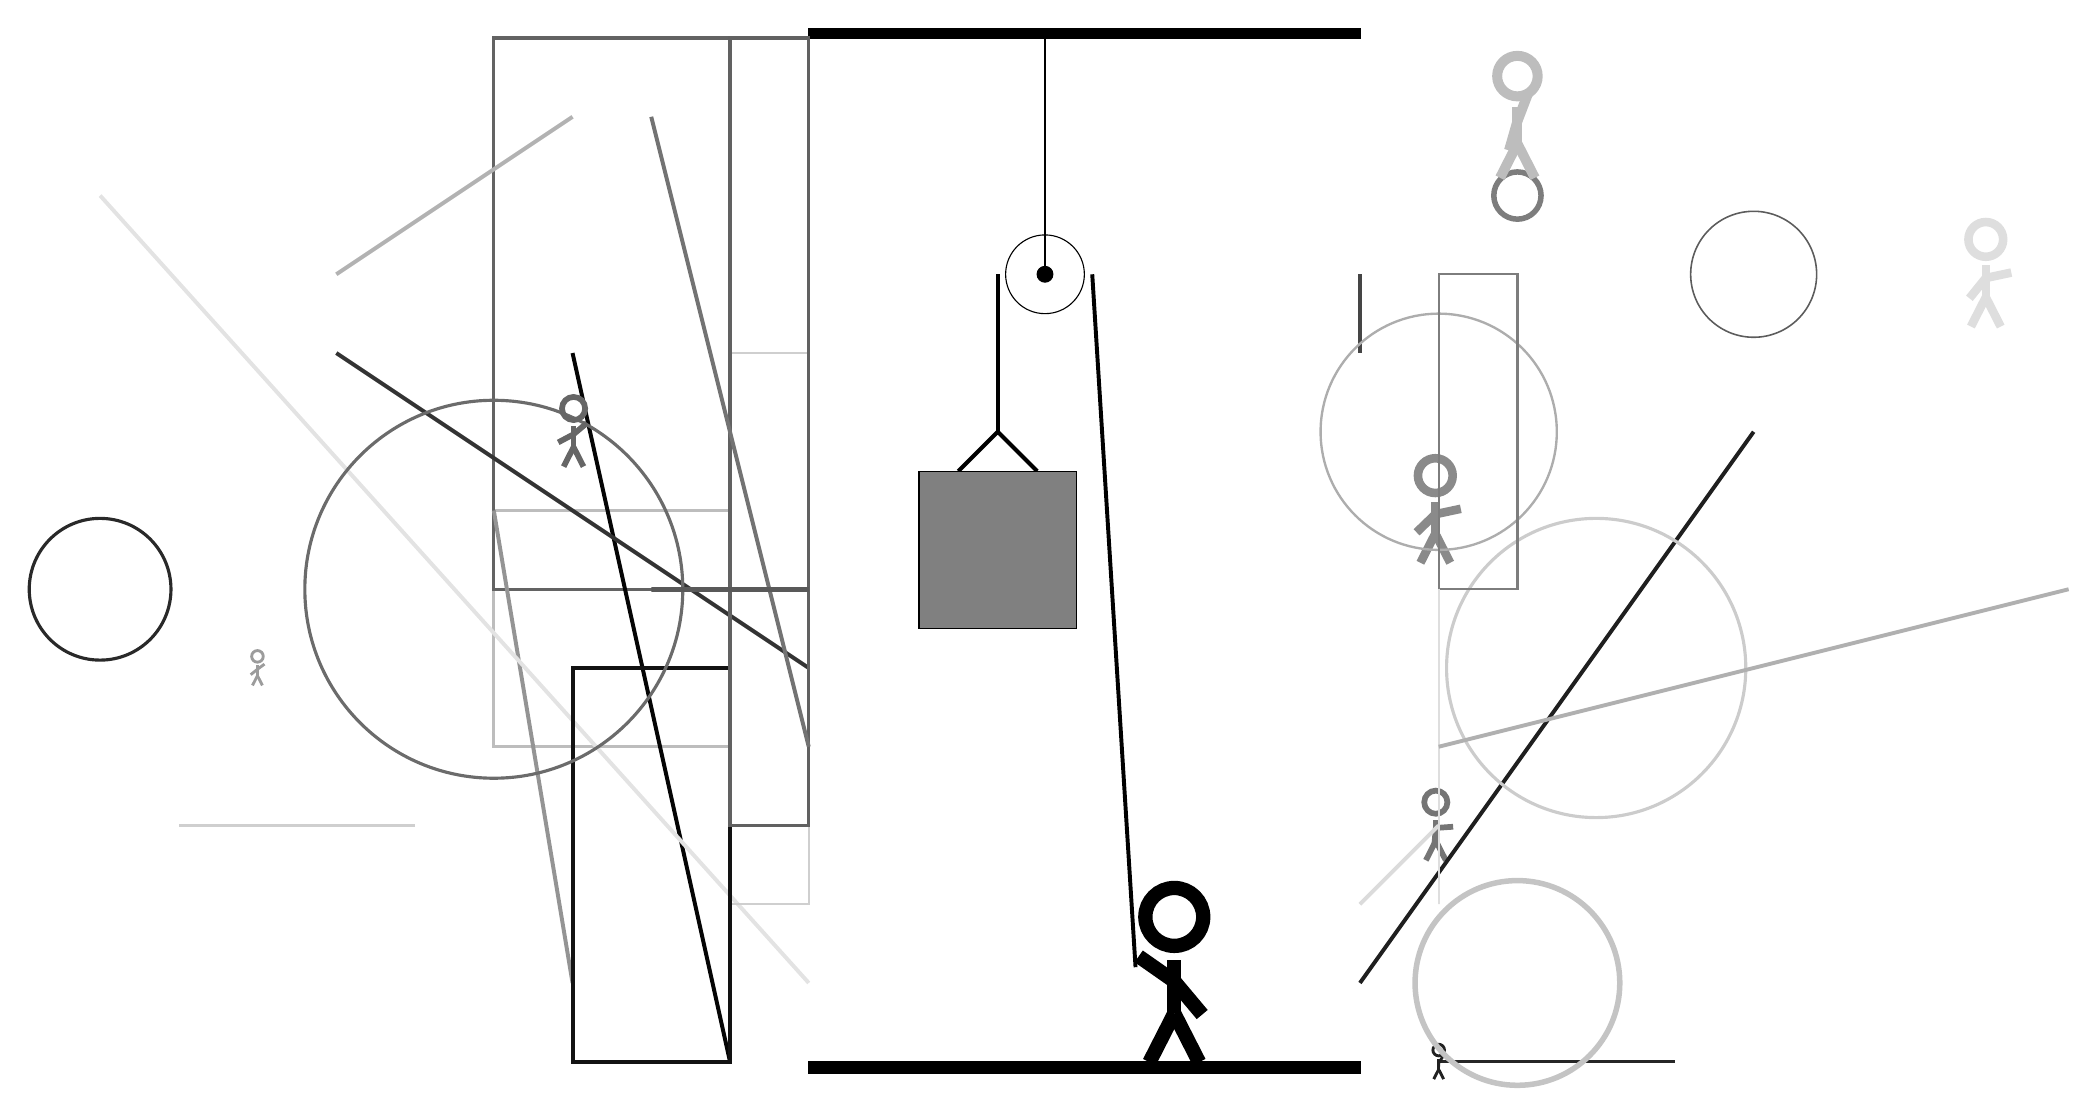
\begin{tikzpicture}
		%%%%% START %%%%%
		
		\draw[fill=black] (-2, 10) rectangle (5, 10.125);
		
		\node[line width=0.3mm, color=black!46] at (6, 4) {\Strichmaxerl[6][44][12]};
		
		\node[line width=0.7mm, color=black!13] at (13, 7) {\Strichmaxerl[6][51][12]};
		\draw[line width=0.4mm, color=black!85] (6, -3) rectangle (9, -3);
		\node[line width=0.2mm, color=black!87] at (6, -3) {\Strichmaxerl[2][88][57]};
		\draw[line width=0.4mm, color=black!26] (-3, 4) rectangle (-6, 1);
		
		\draw[line width=0.4mm, color=black!61] (-3, 10) rectangle (-6, 3);
		
		\draw[line width=0.5mm, color=black!73](5, 7) -- (5, 6);
		\node[line width=0.6mm, color=black!54] at (6, 0) {\Strichmaxerl[4][85][4]};
		\draw[line width=0.5mm, color=black!42](-6, 4) -- (-5, -2);
		\draw [line width=0.3mm, color=black!32](6, 5) circle (1.5);
		\draw[line width=0.5mm, color=black!19](-7, 0) -- (-10, 0);
		
		\node[line width=0.3mm, color=black!39] at (-9, 2) {\Strichmaxerl[2][39][36]};
		\draw[line width=0.5mm, color=black!88](10, 5) -- (5, -2);
		
		\draw[line width=0.5mm, color=black!98](-5, 6) -- (-3, -3);
		\draw[line width=0.5mm, color=black!11](-2, -2) -- (-11, 8);
		\draw[line width=0.2mm, color=black!19] (-3, 6) rectangle (-2, -1);
		
		\draw[line width=0.5mm, color=black!80](-2, 2) -- (-8, 6);
		
		\draw[line width=0.5mm, color=black!14](5, -1) -- (6, 0);
		\draw[line width=0.5mm, color=black!93] (-3, -3) rectangle (-5, 2);
		
		\draw[line width=0.5mm, color=black!30](-5, 9) -- (-8, 7);
		\draw [line width=0.7mm, color=black!23](7, -2) circle (1.3);
		
		\draw [line width=0.7mm, color=black!51](7, 8) circle (0.3);
		\draw [line width=0.4mm, color=black!20](8, 2) circle (1.9);
		\draw[line width=0.3mm, color=black!51] (6, 3) rectangle (7, 7);
		\draw [line width=0.4mm, color=black!58](-6, 3) circle (2.4);
		
		\node[line width=0.2mm, color=black!60] at (-5, 5) {\Strichmaxerl[4][28][40]};
		\node[line width=0.3mm, color=black!26] at (7, 9) {\Strichmaxerl[7][74][69]};
		\draw [line width=0.2mm, color=black!29](13, 2) circle (0.0);
		\draw[line width=0.4mm, color=black!62] (-3, 10) rectangle (-2, 0);
		\draw[line width=0.3mm, color=black!13] (6, -1) rectangle (6, 3);
		\draw[line width=0.5mm, color=black!31](6, 1) -- (14, 3);
		
		\draw[line width=0.5mm, color=black!55](-4, 9) -- (-2, 1);
		\draw [line width=0.4mm, color=black!84](-11, 3) circle (0.9);
		
		\draw[line width=0.6mm, color=black!65] (-2, 3) rectangle (-4, 3);
		\draw [line width=0.2mm, color=black!64](10, 7) circle (0.8);
		
		\draw (1, 7) circle (0.5);
		\draw[fill=black] (1, 7) circle (0.1);
		\draw (1, 10) -- (1, 7);
		
		\draw[line width=0.5mm] (-0.1, 4.5) -- (0.4, 5.0) -- (0.9, 4.5);
		\draw[fill=black!50] (-0.6, 4.5) rectangle (1.4, 2.5);
		
		\draw[line width=0.5mm] (0.4, 7) -- (0.4, 5.0);
		\centerarc[line width=0.5mm](1, 7)(0:180:0.6);
		\draw[line width=0.5mm](1.6, 7) -- (2.15, -1.8);
		
		\node at (2.6, -1.9) {\Strichmaxerl[10][-35][-50]};
		
		\draw[fill=black] (-2, -3) rectangle (5, -3.15);
		
		%%%%% END %%%%%
	\end{tikzpicture}
\end{document}